\documentclass[11pt, a4paper]{article}
\usepackage[T1]{fontenc}
\usepackage[utf8]{inputenc}
\usepackage[MeX]{polski}
\usepackage[polish]{babel}
\usepackage{enumerate}
\usepackage{float}
\usepackage{geometry}
\usepackage{amsmath}
\usepackage[linesnumbered,ruled]{algorithm2e}
\usepackage{graphicx}
\usepackage{caption}


\graphicspath{{../plots/}}

\geometry{top=1.5cm, bottom=1.5cm, right=1.5cm, left=1.5cm}


\title{Obliczenia naukowe\\Lista3}
\author{Stanisław Woźniak}
\date{}

\begin{document}
    \maketitle
    \section{Zadanie 1.}
    \subsection{Metoda Bisekcji}
    \subsection{Opis}
    Jedna z metod znajdowania miejsca zerowego funkcji ciągłej na podanym przedziale.\\
    Metoda polega na połowieniu danego przedziału z każdą iteracją do momentu znalezienia szukanego $x$ z dokładnością do $\delta$ lub do momentu gdy $|f(x)| < \epsilon$
    Z każdą iteracją jest definiowany nowy przedział. Jeden koniec ma w połowie poprzedniego przedziału. Natomiast drugi jest wybierami z dwóch poprzednich z warunkiem, że znak wartości funkcji na krańcach przedziału jest przeciwny.\\
    Warunki początkowe:
    \begin{enumerate}
        \item Badana funkcja posiada miejsce zerowe.
        \item Badan funkcja jest ciągła na przedziale [a,b]
        \item Na krańcach przedziału wartość funkcji musi mieć przeciwne znaki.
    \end{enumerate}
    \subsection{Pseudokod}
    \begin{algorithm}[H]
        \SetKwInOut{Input}{Input}
        \SetKwInOut{Output}{Output}

        \underline{Metoda Bisekcji} $(f, a,b, \delta,\epsilon)$\;
        \Input{f - funkcja, [a,b] - przedział, $\delta$ - dokładność $x_{0}$, $\epsilon$ - dokładność $f(x_{0})$}
        \Output{k, $x_{0}$, $f(x_{0})$}
        $x_{0} \leftarrow 0;k \leftarrow 0$\;
        \While{$|a - b| > \delta$}
        {
            $k++$\;
            \uIf{$f(a)*f(b) < 0$}
            {
                $x_{0} \leftarrow a + \frac{b-a}{2}$\;
            }
            \Else{
                return ''Error: Funkcja nie zmienia znaku w przedziale''\;
            }

            \If{$|f(x_{0})| < \epsilon$}
            {
                return $(k, x_{0}, f(x_{0}))$\;
            }

            \uIf{$f(x_{0})*f(a) < 0$}
            {
                $b \leftarrow x_{0}$\;
            }\ElseIf{$f(x_{0})*f(b) < 0$}
            {
                $a \leftarrow x_{0}$\;
            }
        }
        return $(k, x_{0}, f(x_{0}))$\;
        \caption{Metoda Bisekcji}
    \end{algorithm}
    
    \section{Zadanie 2.}
    \subsection{Metoda Newtona (stycznych)}
    \subsection{Opis}
    Jest to algorytm iteracyjny przybliżajacy pierwiastek funkcji. Metoda polega na wyprowadzaniu stycznych z wybranego punktu $f(x_{0})$. Punkt przecięcia stworzonej stycznej z osią OX jest szukanym miejsciem zerowym. Jeśli się okaże, ze przybliżenie jest zbyt mało dokładne czynność jest powtarzana gdzie do $x_{0}$ przypisuje się wyznaczone poprzednio miejsce zerowe. 
    \subsection{Pseudokod}
    \begin{algorithm}[H]
        \SetKwInOut{Input}{Input}
        \SetKwInOut{Output}{Output}

        \underline{Metoda Bisekcji} $(f, f',x_{0}, \delta,\epsilon, maxit)$\;
        \Input{f - funkcja, f' - pochodna funkcji, $x_{0}$ - przybliżenie początkowe, $\delta$ - dokładność $x_{0}$, $\epsilon$ - dokładność $f(x_{0})$, maxit - maksymalna liczba iteracji}
        \Output{k, $x_{0}$, $f(x_{0})$}
        $k \leftarrow 0; x_{1} \leftarrow x_{0} - 1; v \leftarrow f(x_{0})$\;
        \While{$|x_{1} - x_{0}|> \delta$}
        {
            $k++$\;
            \If{$k > maxit$}
            {
                return ''Error: Przekroczenie liczby iteracji''\;
            }
            \If{$|f'(x_{0})| < \epsilon$}
            {
                return ''Error: Pochodna bliska zeru''\;
            }

            $x_{1} \leftarrow x_{0}; x_{0} \leftarrow x_{0} - \frac{v}{f'(x_{0})}; v \leftarrow f(x_{0})$\;

            \If{$|v| < \epsilon$}
            {
                return $(k, x_{0}, v)$\;
            }
        }
        return $(k, x_{0}, v)$\;
        \caption{Metoda Newtona}
    \end{algorithm}
    \section{Zadanie 3.}
    \subsection{Metoda Siecznych}
    \subsection{Opis}
    Metoda wyznaczania przybliżenia miejsca zerowego funkcji. W tym algorytmi przyjmuje się, że podana funkcja jest ciągła, oraz na dostatecznie małym odcinku w przybliżeniu zmienia się w sposób liniowy. To założenie pozwala nam zastąpić dany fragment wykresu funkcji sieczną. Punkt przecięcia siecznej z osią OX jest szukanym przybliżeniem miejsca zerowego. Jeśli przybliżenie nie jest wystarczająco dokładne, czynność zostaje powtarzana przyjmując punkt wyliczony w poprzedniej iteracji jako koniec siecznej.
    
    Warunek powodzenia:\\
    
    $$\bigwedge_{n>0} (f(x_{n})f(x_{n-1}) < 0) $$
    
    \subsection{Pseudokod}
    \begin{algorithm}[H]
        \SetKwInOut{Input}{Input}
        \SetKwInOut{Output}{Output}

        \underline{Metoda Siecznych} $(f, x_{0},x_{1}, \delta,\epsilon, maxit)$\;
        \Input{f - funkcja, $x_{0}, x_{1}$ - przybliżenia początkowe, $\delta$ - dokładność $x_{0}$, $\epsilon$ - dokładność $f(x_{0})$, maxit - maksymalna liczba iteracji}
        \Output{k, $x_{0}$, $f(x_{0})$}
        $fa \leftarrow f(x_{0}); fb \leftarrow f(x_{1}); k \leftarrow 0$\;
        \While{$|x_{1} - x_{0}| > \delta$}
        {
            $k++$\;
            \If{$k > maxit$}
            {
                return ''Error: Przekroczenie liczby iteracji''\;
            }

            \If{$|fa| > |fb|$}
            {
                $x_{0} \leftrightarrow x_{1}; fa \leftrightarrow fb$\;
            }

            $s \leftarrow \frac{(x_{0} - x_{1})}{fb - fa}$\;
            $x_{1} \leftarrow x_{0}; fb \leftarrow fa$\;
            $x_{0} \leftarrow x_{0} - fa*s; fa \leftarrow f(x_{0})$\;
            \If{$|fa| < \epsilon$}
            {
                return $(k, x_{0}, fa)$\;
            }
        }
        return $(k, x_{0}, fa)$\;
        \caption{Metoda Siecznych}
    \end{algorithm}
    \section{Zadanie 4.}
    \subsection{Problem}
    Problem polegał na wyznaczeniu pierwiastka równania przy użyciu zaimplementowanych metod w poprzednich zadaniach.
    
    Równanie:
    \[\sin{x} - (\frac{1}{2}x)^{2} = 0 \]

    Dla każdej z metod zostały użyte te same dokładności $\delta$ oraz $\epsilon$ równe $\frac{1}{2} * 10^{-5}$.\\
    Jednakże początkowe przybliżenia oraz przedziały dla każdej z nich zostały zdefiniowane inne.
    \begin{enumerate}
        \item Metoda bisekcji - przedział początkowy $[1.5, 2]$
        \item Metoda Newtona (Metoda stycznych) - przybliżenie początkowe $x_{0} = 1.5$
        \item Metoda siecznych - przybliżenia poczatkowe $x_{0} = 1$, $x_{1} = 2$
    \end{enumerate}
    \subsection{Wyniki}
    Na potrzeby rozwiązania równania danymi metodami lewa strona równania została uznana za funkcję f
    Oznaczenia:\\
    r - znalezione miejsce zerowe z dokładnością do $\delta$ \\
    v - wartość funkcji w punkcie r z dokładnością do $\epsilon$ \\
    it - liczba wykonanych iteracji potrzebnych do znalezienia pierwiastka \\
    err - powiadomienie o błędzie

    Prawidłowy wynik: $r_{0} = 0$, $r_{1} = 1.93375$, $v_{0} = v_{1} = 0$.
    \begin{center}
        \begin{tabular}{c|c|c|c|c}
            metoda & r & v & it & err\\
            \hline
            bisekcji & 1.9337539672851562 & -2.7027680138402843e-7 & 16 & Brak błędu\\
            stycznych & 1.933749984135789 & 4.995107540040067e-6 & 13 & Brak błędu\\
            siecznych & 1.933753644474301 & 1.564525129449379e-7 & 4 & Brak błędu\\
        \end{tabular}
    \end{center}
    \subsection{Wnioski}
    Analizując wyniki, można zauważyć, że każda z metod podała jeden z dwóch prawidłowych pierwiastków. Metoda bisekcji nie podała drugiego ponieważ w podanym przedziale znajdował się tylko jeden, ale także dlatego, że algorytm działa poprawnie, kiedy w przedziale (początkowym lub stworzonym w czasie działania algorytmu) znajduje się nieparzysta ilość pierwiastków (tzn. wartości funkcji na krańcach przedziału mają różne znaki). Natomiast metoda stycznych znalazła pierwiastek najbliższy w kierunku zbieżności, ponieważ przybliżenie początkowe było ustalone w taki sposób, że metoda Newtona z tego punktu zbiegała do pierwiastka $r_{1}$. Metoda siecznych wyznaczyła także to samo miejsce zerowe, ponieważ przybliżenia początkowe zostały tak dobrane, że pomiędzy nimi był tylko jeden punkt zerowy. Jednakże metoda siecznych nie działałaby poprawnie gdyby pomiędzy tymi punktami znalazłby się także drugi pierwiastek, gdyż założeniem poprawności tejmetody jest, że wartości funkcji na podanych przybliżeniach są różnego znaku.

    Porównując wartości z tabeli także można zauważyć, że metoda bisekcji do znalezienia pierwiastka potrzebowała najwiecej iteracji. Zachodzi takie zjawisko, ponieważ metoda bisekcji ma zbieżność liniową, natomiast metody Newtona i siecznych mają zbieżność kwadratową.

    \section{Zadanie 5.}
    \subsection{Problem}
    Zadanym problemem było znaleźć punkty przecięcia się wykresów dwóch funkcji.
    \begin{enumerate}
        \item $f(x) = 3x$
        \item $g(x) = e^{x}$
    \end{enumerate}
    Dokładność obliczeniowe wynosiły: $\delta = \epsilon = 10^{-4}$\\
    Aby znaleźć odpowiednie punkty przecięcia należało stworzyć funkcję pomocniczą h.
    \[h(x) = f(x) - g(x)\]
    Ten sposób zapewniał znalezienie punkty przeciecia wykresów funkcji f oraz g metodą znalezienia miejsc zerowych funkcji h.\\
    Do znalezienia rozwiązania należało użyć metodę bisekcji.
    \subsection{Wyniki}
    [a,b] - przedział początkowy \\
    r - znalezione miejsce zerowe z dokładnością do $\delta$ \\
    v - wartość funkcji w punkcie r z dokładnością do $\epsilon$ \\
    it - liczba wykonanych iteracji potrzebnych do znalezienia pierwiastka \\
    err - powiadomienie o błędzie

    Prawidłowy wynik (przybliżony): $r_{1}$ = 0.619061, $r_{2}$ = 1.51213.
    \begin{figure}[H]
        \caption{Funkcja h}
        \centering
        \begin{minipage}{0.4\textwidth}
            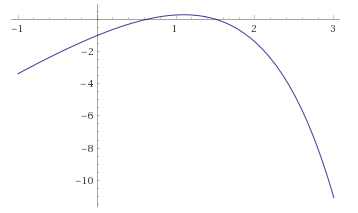
\includegraphics[width=\linewidth]{zad5}
        \end{minipage}
    \end{figure}
    \begin{center}
        \begin{tabular}{c|c|c|c|c}
            [a, b] & r & v & it & err\\
            \hline
            $[0.5, 0.7]$ & 0.619140625 & 9.066320343276146e-5 & 9 & Brak błędu\\
            $[-1, 1]$ & 0.619140625 & 9.066320343276146e-5 & 10 & Brak błędu\\
            $[0.0, 1.5]$ & 0.61907958984375 & 2.091677592419572e-5 & 13 & Brak błędu\\
            $[1, 2]$ & 1.5120849609375 & 7.618578602741621e-5 & 13 & Brak błędu\\
            $[1.5, 1.7]$ & 1.512109375 & 3.868007140983565e-5 & 9 & Brak błędu\\
            $[-1, 2]$ & - & - & - & Funkcja nie zmienia znaku na przedziale [a,b]\\
            $[-10, 0]$ & - & - & - & Funkcja nie zmienia znaku na przedziale [a,b]\\
            $[1, 1.5]$ & - & - & - & Funkcja nie zmienia znaku na przedziale [a,b]\\
            $[2, 10]$ & - & - & - & Funkcja nie zmienia znaku na przedziale [a,b]
        \end{tabular}
    \end{center}
    \subsection{Wnioski}
    Przedziały, które zostały podane w tabeli zostały dobrane po obserwacji wykresu. Po wynikach można zaobserwować, że metoda bisekcji poprawnie znajduje pierwiastki tylko jesli prawidłowo zdefiniujemy przedziały. Można także zaobserwować różnice w wynikach. Jeśli wyliczony pierwiastek różni się o więcej niż $\delta$ od wyliczonego (tego samego) pierwiastka zaczynając z innego przedziału, wtedy wartość w pierwiastku ($h(r)$) jest dokładny do $\epsilon$. Także można zaobserwować, że ilość iteracji nie jest zawsze zależna od wielkości przedziału. Dzieje się to dlatego, że może się zdarzyć, że przy połowieniu jednego przedziału znajdzie się szukane miejsce, gdy w przypadku wyliczania pierwiastka zaczynając z drugim przedziałem skończy się iteracje przy przedziale < $\delta$. 

    W tym zadaniu pokazane zostało, że metoda bisekcji nie jest dobrą metodą w przypadku gdy nie znamy przedziałów funkcji, w których jest tylko jedno miejsce zerowe. Po wynikach możemy zauważyć, że źle dobrane przedziały zwrócą błąd zamiast poprawnego wyniku. Można temu zapobiec przez użycie innej metody, która nie potrzebuje znajomości zmiany znaku w wartościach funkcji, albo tak jak opisane zostało powyżej, wywołanie metody bisekcji po poprzednio przeanalizowaniu wykresu funkcji.

    \section{Zadanie 6.}
    \subsection{Problem}
    Należało znaleźć miejsca zerowe trzema metodami (bisekcji, stycznych oraz siecznych) dwóch funkcji:
    \begin{enumerate}
        \item $f(x) = e^{1-x} - 1$ (prawidłowe rozwiązanie: x = 1)
        \item $g(x) = xe^{-x}$ (prawidłowe rozwiązanie: x = 0)
    \end{enumerate}
    Obliczenia należało wykonać z dokłądnością $\delta = \epsilon = 10^{-5}$\\
    Także zadaniem było dobrać odpowiedni przedział i przybliżenia początkowe.
    \subsection{Wyniki}
    \begin{figure}[H]
        \caption{Funkcja f}
        \begin{minipage}{0.4\textwidth}
            \centering
            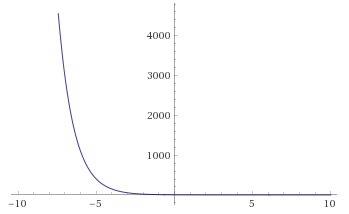
\includegraphics[width=\linewidth]{fminus10to10}
        \end{minipage}
        \begin{minipage}{0.4\textwidth}
            \centering
            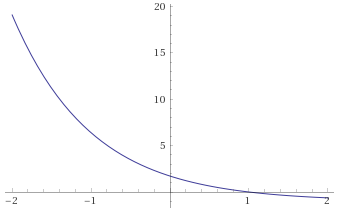
\includegraphics[width=\linewidth]{fminus2to2}
        \end{minipage}
    \end{figure}
    \begin{figure}[H]
        \caption{Funkcja g}
        \begin{minipage}{0.4\textwidth}
            \centering
            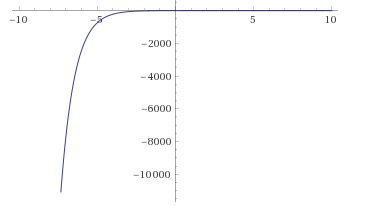
\includegraphics[width=\linewidth]{gminus10to10}
        \end{minipage}
        \begin{minipage}{0.4\textwidth}
            \centering
            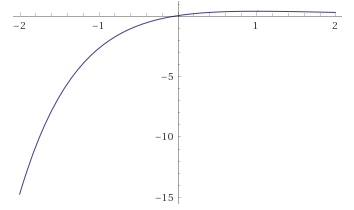
\includegraphics[width=\linewidth]{gminus2to2}
        \end{minipage}
    \end{figure}

    r - znalezione miejsce zerowe z dokładnością do $\delta$ \\
    v - wartość funkcji w punkcie r z dokładnością do $\epsilon$ \\
    it - liczba wykonanych iteracji potrzebnych do znalezienia pierwiastka \\
    err - powiadomienie o błędzie

    \begin{center}
        \begin{tabular}{|c|c|c|c|c|c|}
            \hline
            \multicolumn{6}{|c|}{Metoda bisekcji}\\
            \hline
            funkcja & [a,b] & r & v & it & err\\
            \hline
            f & $[0.5, 2]$ & 0.9999923706054688 & 7.629423635080457e-6 & 16 & Brak błędu\\
            f & $[-0.1, 2]$ & 1.0000038146972656 & -3.814689989667386e-6 & 17 & Brak błędu\\
            f & $[0.0, 2]$ & 1.0 & 0.0 & 1 & Brak błędu\\
            f & $[-100, 100]$ & 0.9999990463256836 & 9.536747711536009e-7 & 23 & Brak błędu\\
            f & $[0.99999, 20]$ & 1.0000081198215485 & -8.119788582838794e-6 & 20 & Brak błędu\\
            \hline
            g & $[-0.5, 1]$ & -7.62939453125e-6 & -7.629452739132958e-6 & 16 & Brak błędu\\
            g & $[-0.5, 0.5]$ & 0.0 & 0.0 & 1 & Brak błędu\\
            g & $[-0.1, 4]$ & 3.8146972656107834e-6 & 3.8146827137233106e-6 & 17 & Brak błędu\\
            g & $[-100, 101]$ & 4.410743713378906e-6 & 4.410724258761706e-6 & 23 & Brak błędu\\
            \hline
        \end{tabular}
    \end{center}
    
    \begin{center}
        \begin{tabular}{|c|c|c|c|c|c|}
            \hline
            \multicolumn{6}{|c|}{Metoda Newtona}\\
            \hline
            funkcja & x0 & r & v & it & err\\
            \hline
            f & 4 & 0.9999999995278234 & 4.721765201054495e-10 & 21 & Brak błędu\\
            f & 2 & 0.9999999810061002 & 1.8993900008368314e-8 & 5 & Brak błędu\\
            f & 11 & NaN & NaN & 2 & Wyjście poza zakres\\
            f & 101 & NaN & NaN & 1 & Pochodna bliska zeru\\
            \hline
            g & -1 & -3.0642493416461764e-7 & -3.0642502806087233e-7 & 5 & Brak błędu\\
            g & 1 & NaN & NaN & 1 & Pochodna bliska zeru\\
            g & 2 & 14.398662765680003 & 8.036415344217211e-6 & 10 & Brak błędu\\
            g & 11 & 14.272123938290518 & 9.040322779745372e-6 & 3 & Brak błędu\\
            g & 101 & NaN & NaN & 1 & Pochodna bliska zeru\\
            \hline
        \end{tabular}
    \end{center}

    \begin{center}
        \begin{tabular}{|c|c|c|c|c|c|c|}
            \hline
            \multicolumn{7}{|c|}{Metoda siecznych}\\
            \hline
            funkcja & x1 & x2 & r & v & it & err\\
            \hline
            f & 0.5 & 2 & 1.000000014307199 & -1.4307198870078253e-8 & 6 & Brak błędu\\
            f & -0.1 & 2 & 1.0000032272298756 & -3.227224668056472e-6 & 6 & Brak błędu\\
            f & 0 & 2 & 1.0000017597132702 & -1.7597117218937086e-6 & 6 & Brak błędu\\
            f & -100 & 101 & 101.0 & -1.0 & 1 & Brak błędu\\
            f & 0.99999 & 20 & 1.0000000009000212 & -9.000211687038018e-10 & 2 & Brak błędu\\
            \hline
            g & -1 & 0.5 & -1.1737426154042664e-6 & -1.1737439930768023e-6 & 7 & Brak błędu\\
            g & -0.5 & 0.5 & 5.38073548562323e-6 & 5.380706533386756e-6 & 6 & Brak błędu\\
            g & -0.1 & 4 & 14.32970132001514 & 8.568936563065177e-6 & 14 & Brak błędu\\
            g & -100 & 101 & 101.0 & 1.3822248658855914e-42 & 1 & Brak błędu\\
            \hline
        \end{tabular}
    \end{center}
    \subsection{Wnioski}
    Obserwując wykresy obu podanych funkcji możemy odpowiednio dobrać przybliżenia początkowe. Natomiast porównując wyniki możemy zaobserwować różnice w dokładnościach metod oraz błędy w zależności od dobranych parametrów.

     Metoda bisekcji, jak można zauważyć po wynikach w tabeli, w każdym testowanym przypadku znajdował prawidłowy wynik z dokładnością do $\delta$. Jednakże porównując do pozostałych metod można zaobserwować, że algorytm potrzebuje najwiekszej liczby iteracji do wyznaczenia odpowiedniego wyniku. Dzieje się to dlatego, że metoda bisekcji zbiega liniowo, kiedy to metody Newtona i siecznych mają rząd 2, czyli zbiegają kwadratowo.

     Można zauważyć, że metoda Newtona przy pewnych przybliżeniach początkowych nie zbiega do wartości liczbowej. Dzieje się to dlatego, że przy wybraniu pewnych parametrów metoda ta jest rozbieżna, co oznacza, że każdy kolejny punkt sprawdzanej stycznej odbiega od szukanego miejsca zerowego. Patrząc na błędy, które pojawiają się w przypadkach rozbieżności możemy zauważyć, że iterując po kolejnych punktach stycznych do wykresu wyszliśmy poza zakres Float64 co oznacza, że metoda jest rozbieżna. W innym przypadku metoda nie zbiega do wartości liczbowej ponieważ pochodna w znalezionym punkcie była bliska zeru, co oznacza także rozbieżność metody. 

     W przypadku metody siecznych, obserwując wyniki można zauważyć zauważyć, że przy funkcji $g$ wartości r znacznie się od siebie różnią. Można wytłumaczyć to obserwując wykres oraz analizując algorytm. Algorytm kończy swoje działanie gdy znajdzie $g(x) < \epsilon$. $\epsilon$, który został użyty do obliczeń był dokładności $10^{-5}$. Natomiast w tabeli widzimi wartości funkcji $g$ w punktach r, które są poniżej $\epsilon$. Z tego wynika, że algorytm zadziałał poprawnie, ale wyniki odbiegają od rzeczywistego miejsca zerowego z powodu precyzji obliczeń. W przypadku funkcji $f$ większość wyników jest prawidłowa z dokładnością do $\delta$ co oznacza, że metoda poprawnie działa dla podanych punktów poczatkowych. Jeden z testowanych przedziałów ma znacznie różniący się wynik od pozostałych. Analizując wykres można wywnioskować dlaczego tak się dzieje. Otóż algorytm działa w taki sposób, że tworzy sieczną pomiędzy danymi punktami. Punkt potrzebny do kolejnej iteracji jest ustalany poprzez sprawdzenie w którym punkcie wyznaczona sieczna przecina oś OX. Gdy spojrzy się na wykres można zauwazyć, że $f(-100)$ oraz $f(101)$ leża na układzie współrzędnych względem siebie w takich punktach, że gdy poprowadzi się sieczną pomiędzy tymi punktami, punkt przecięcia osi OX przez sieczną jest nadal w punkcie $x_{0} = 101 + \delta$. Takie zjawisko sprawia, że algorytm zadziałał poprawnie, lecz zwrócił nieprawidłowy wynik.

\end{document}